\documentclass[11pt, oneside]{article} 
\usepackage{amsmath, amsthm, amssymb, calrsfs, wasysym, verbatim, bbm, color, graphics, graphicx, geometry}
\usepackage[most]{tcolorbox}
\usepackage{xcolor}
\usepackage{framed}
\usepackage{caption}
\usepackage{subcaption}
%\colorlet{shadecolor}{blue!15}
\graphicspath{ {./figs} }

\geometry{tmargin=.75in, bmargin=.75in, lmargin=.75in, rmargin = .75in}  

\newcommand{\R}{\mathbb{R}}
\newcommand{\C}{\mathbb{C}}
\newcommand{\Z}{\mathbb{Z}}
\newcommand{\N}{\mathbb{N}}
\newcommand{\Q}{\mathbb{Q}}
\newcommand{\Cdot}{\boldsymbol{\cdot}}

%\newtheorem{thm}{Theorem}
%\newtheorem{defn}{Definition}
%\newtheorem{conv}{Convention}
%\newtheorem{rem}{Remark}
%\newtheorem{lem}{Lemma}
%\newtheorem{cor}{Corollary}
%\newtheorem{exa}{Ejemplo}

\newtcbtheorem[auto counter]{eje}%
  {Ejemplo}{fonttitle=\bfseries\upshape, fontupper=\slshape,
     arc=0mm, colback=blue!5!white,colframe=blue!75!black}{Ejemplo}

\newtcbtheorem[auto counter]{alg}%
  {Algoritmo}{fonttitle=\bfseries\upshape, fontupper=\slshape,
     arc=0mm, colback=red!5!white,colframe=red!75!black}{Algoritmo}

\title{Estructuras Hidr\'aulicas [2015961] \\ \textbf{Tema \# 3: Flujo variado}}
\author{\textbf{Luis Alejandro Morales, Ph.D}\\ \vspace{0.4cm} Profesor Asistente \\ Universidad Nacional de Colombia-Bogot\'a\\Facultad de Ingenier\'ia \\ Departamento de Ingenieria Civil y Agr\'icola}
%\date{Periodo 2022-II}
\date{}

\begin{document}

\maketitle
\tableofcontents

%\vspace{.25in}

%%%%%%%%
\section{Introducci\'on} % From Chau 
En canales naturales la pendiente y la secci\'on transversal cambian a lo largo del canal, lo cual ocurre tambi\'en en canales arficiales en donde, por razones constructivas y de la topograf\'ia del terreno, la pendiente y la secci\'on cambian mediante estructuras de transici\'on.  Esto hace que el flujo cambie constantemente y que el flujo sea \emph{no uniforme}. Si el cambio  en la l\'amina de agua a lo largo del canal es relativamente  pequeño se le conoce como \emph{flujo gradualmente variado (FGV)}, si el cambio es fuerte, se le conoce como \emph{flujo rapidamente variado (FRV)}. El FGV se analisa para secciones largas de canales por lo que es necesario considerar las p\'erdidas de energ\'ia debido a la fricci\'on. Sin embargo, teniendo en cuenta que el  FRV se presenta en secciones cortas de un canal, las p\'erdidas de energ\'ia por fricci\'on son despreciables. Teniendo en cuenta que las l\'ineas de flujo en el FGV son c\'asi paralelas y siguen una trayectoria c\'asi recta, una distribuci\'on de presiones hidroest\'atica es considerada all\'i. En el FRV, los fuertes gradientes del flujo generan curvaturas de las l\'ineas de corriente y por lo tanto aceleraciones en direcci\'on normal al flujo por lo que considerar una distribuci\'on hidroestatica de presiones no es correcto. 

%En flujo a superficie libre actuan basicamente dos fuerzas: \emph{fuerzas gravitacionales} cuya componente en direcci\'on del flujo en un canal de pendiente positiva acelera el flujo hacia abajo, y las \emph{fuerzas de fricci\'on} debido a la rugosidad del canal que tratan de frenar el flujo. Note que en un canal con pendiente negativa, el flujo trata de desacerelarse. En un canal con pendiente positiva, si las fuerzas de fricci\'on son mayores que las fuezas gravitacionales, el flujo se sesacelera produciendo una elevacion de la lamina de agua, lo cual se da gracias al principio de \emph{coservacion de la masa}. En el caso contrario la profundidad de la lamina de agua disminuye y la velocidad aumenta. En canales prismaticos largos, es posible que las dos fuerzas se igualen en alguna secci\'on del canal haciendo que ni la profundidad ni la velocidad cambien a partir de este punto aguas abajo (ver figura~\ref{fig1}). Por lo tanto, en un flujo en el cual la profundidad no cambia se le denomina \emph{flujo uniforme} y a la profundidad del flujo \emph{profundidad normal}.
%En flujo a superficie libre actuan basicamente dos fuerzas: \emph{fuerzas gravitacionales} cuya componente en direcci\'on del flujo en un canal de pendiente positiva acelera el flujo hacia abajo, y las \emph{fuerzas de fricci\'on} debido a la rugosidad del canal que tratan de frenar el flujo. Note que en un canal con pendiente negativa, el flujo trata de desacerelarse. En un canal con pendiente positiva, si las fuerzas de fricci\'on son mayores que las fuezas gravitacionales, el flujo se sesacelera produciendo una elevacion de la lamina de agua, lo cual se da gracias al principio de \emph{coservacion de la masa}. En el caso contrario la profundidad de la lamina de agua disminuye y la velocidad aumenta. En canales prismaticos largos, es posible que las dos fuerzas se igualen en alguna secci\'on del canal haciendo que ni la profundidad ni la velocidad cambien a partir de este punto aguas abajo (ver figura~\ref{fig1}). Por lo tanto, en un flujo en el cual la profundidad no cambia se le denomina \emph{flujo uniforme} y a la profundidad del flujo \emph{profundidad normal}.

\section{Flujo gradualmente variado} % From Chau
\subsection{Ecuaciones para el calculo} 
A continuaci\'on se derivan las ecuaciones de FGV para una canal prism\'atico, a partir de las siguientes suposiciones:
\begin{itemize}
    \item Pendiente del fondo del canal pequeña. Esto implica que $\sin \theta \approx \tan \theta \approx \theta$, donde $\theta$ es el angulo del fondo del canal con respecto a la horizontal. 
    \item No hay entradas ni salidas de flujo del canal.
    \item La distribuci\'on de presiones es hidroest\'atica en todas las secciones del canal.
    \item Las perdidas de energia debido a la fricci\'on son calculadas usando alguna de las ecuaciones mencionadas para flujo uniforme.
\end{itemize}
Teniendo en cuenta lo anterior y la figura~\ref{fig1}, la cabeza total de energ\'ia en una secci\'on de canal es:
% Chau fig 5.1
\begin{figure}[h]
\centering
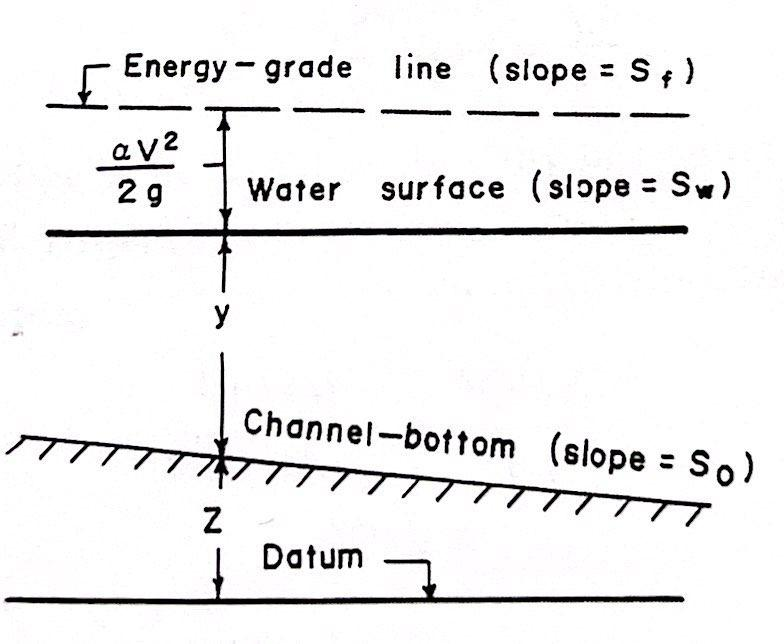
\includegraphics[width=8cm]{fig51.jpeg}
\caption{Secci\'on de flujo gradualmente variado en canal prismatico (tomado de \cite{Chau}).}
\label{fig1}
\end{figure}

\begin{equation}
    H = z + y + \alpha\frac{ V^2}{2g}
\label{eq1}
\end{equation}

en donde $H$ es la elevaci\'on de la l\'inea de energ\'ia con respecto a un nivel de referencia, $z$ es la elevaci\'on del fondo del canal, $y$ es la profundidad de la l\'amina de agua, $V$ es la velocidad media del flujo en la secci\'on transversal y $\alpha$ es el factor de correcci\'on de la energ\'ia cin\'etica. Consideremos $x$ como la distancia  positiva en direcci\'on del flujo. Derivando la ecuaci\'on~\ref{eq1} con respecto a $x$, tenemos:

\begin{equation}
    \frac{dH}{dx} = \frac{dz}{dx} + \frac{dy}{dx} + \frac{\alpha Q^2}{2g} \frac{d}{dx}\left( \frac{1}{A^2}\right)
\label{eq2}
\end{equation}

Por defici\'on, se tiene que $\frac{dH}{dx} = -S_f $ y $\frac{dz}{dx} = -S_o $, donde $S_f$ es la pendiente de la l\'inea de energ\'ia y $S_o$ es la pendiente del fondo del canal; note que el signo negativo indica que las cantidades decrecen a lo largo del canal en direcci\'on del flujo.

Resolviendo:

\begin{equation}
\begin{split}
    \frac{d}{dx}\left( \frac{1}{A^2}\right) & = \frac{d}{dA}\left( \frac{1}{A^2}\right) \frac{dA}{dx} \\
                                            & = \frac{-2}{A^3} \frac{dA}{dy} \frac{dy}{dx} \\
                                            & = \frac{-2B}{A^3}  \frac{dy}{dx}
\end{split}
\label{eq3}
\end{equation}

donde $B = \frac{dA}{dy}$ representa el ancho del canal en la superficie. Para canales no prism\'aticos:
$$
\frac{dA}{dx} = \frac{\partial A}{\partial x} + \frac{\partial A}{\partial y} \frac{\partial y}{\partial x}
$$

Lo que signigica que $A$ cambia en $x$ y $y$. 

Reemplazando terminos en la ecuaci\'on~\ref{eq2} y organizando terminos:

\begin{equation}
    \frac{dy}{dx} = \frac{S_o - S_f }{1-\left(\alpha B Q^2 \right) /\left(g A^3 \right)}
\label{eq4}
\end{equation}

El termino $\frac{\alpha B Q^2 }{g A^3} $ puede ser expresado en funcion del n\'umero de Froude ($F_r$) as $\frac{\alpha B Q^2 }{g A^3}  = \frac{\left(Q/A \right)^2}{\left( gA \right)/\left( \alpha B \right) } = F_r^2 $. De acuerdo con esto, la ecuaci\'on~\ref{eq4}, se expresa como:

\begin{equation}
    \color{red}\boxed{\color{black}   \frac{dy}{dx} = \frac{S_o - S_f }{1-F_r^2}}
\label{eq5}
\end{equation}

La ecuaci\'on~\ref{eq5} es utilizada para analisar el FGV en canales prism\'aticos, su soluci\'on proporciona las profundidades a lo largo de un tramo de canal. Es adem\'as usada para la descripci\'on cualitativa del FGV. 

\subsection{Clasificaci\'on de los perfiles de flujo}
Para clasificar los perfiles de la l\'amina de agua es necesario, en principio, clasificar la pendiente del fondo del canal como:
\begin{itemize}
    \item Pendiente suave (en Ingl\'es, mild) ($M$): Si el flujo uniforme es subcr\'itico ($y_n > y_c$) la pendiente el canal es tipo $M$.
    \item Pendiente alta (en Ingl\'es, steep) ($S$): Si el flujo uniforme es supercr\'itico ($y_n < y_c$) la pendiente del canal es tipo $S$.
    \item Pendiente critica (en Ingl\'es, critical) ($C$): Si el flujo uniforme es cr\'itico ($y_n = y_c$), la pendiente del canal es tipo $C$.
    \item Pendiente horizontal (en Ingl\'es, horizontal) ($H$) : Matem\'aticamente, se puede demostrar que la profundidad normal es infinita si la pendiente es horizontal (tipo $H$).$A R ^{2/3} = \frac{Q n}{S_o}$ incrementa hacia el infinito si $S_o \rightarrow 0$. 
    \item Pendiente adversa (en Ingl\'es, adverse) ($A$): Matem\'aticamente, se puede demostrar que la profundidad normal no existe si la pendiente es adversa (tipo $A$). $A R ^{2/3} = \frac{Q n}{S_o}$ se vuelve negativa (imposible!) si $S_o$ es negativa.
\end{itemize}

La esquematizaci\'on de los perfiles de agua $M$ y $S$ se hace con base en la figura~\ref{fig2}, en donde $NDL$ indica la posici\'on de la profundidad normal (normal-depth line) y $CDL$ indica la posici\'on de la profundidad cr\'itica (critical-depth line). En esta figura se tienen tres zonas que determinan la posici\'on del perfil $M$ o $S$. Note adem\'as, que las posici\'on de $NDL$ y $CDL$ cambia dependiendo de la pendiente del canal (o tipo de flujo). Para los perfiles $C$, $H$, y $A$, teniendo en cuenta que $y_n$ no existe of es igual a $y_c$, existen \'unicamente dos zonas en donde se ubican estos perfiles. 

% Chau fig 5.2
\begin{figure}[h]
\centering
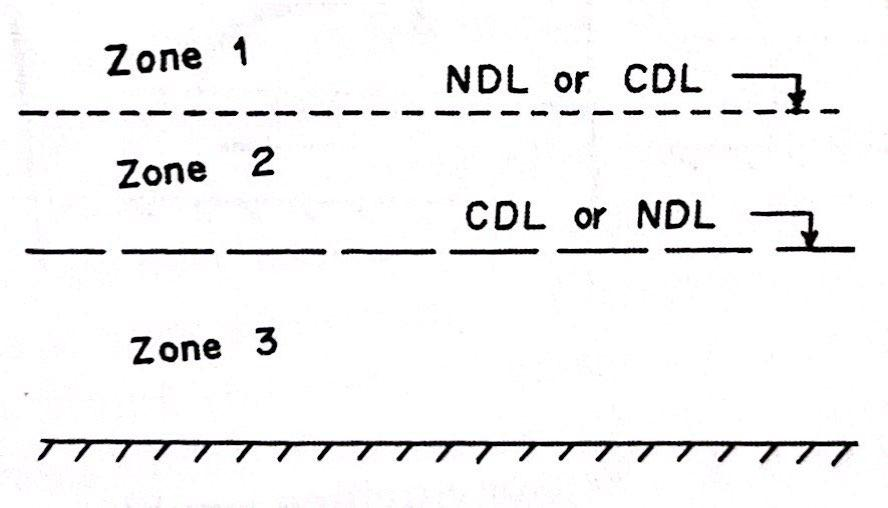
\includegraphics[width=8cm]{fig52.jpeg}
\caption{Zonas para la clasificaci\'on de perfiles de flujo (tomado de \cite{Chau}).}
\label{fig2}
\end{figure}

De acuerdo con lo anterior, se tienen entonces 12 diferentes perfiles de l\'amina de agua: tres para $M$, tres para $S$, dos para $C$ (la zona 2 no existe ya que $y_n = y_c$), dos para $H$ (la zona 1 no existe ya que $y_n = \infty$) y dos para $A$ (la zona 1 no existe ya que $y_n$ no existe). La figura~\ref{fig3} muestra los perfiles de la l\'amina de agua.

% Chau fig 5.3
\begin{figure}[h]
\centering
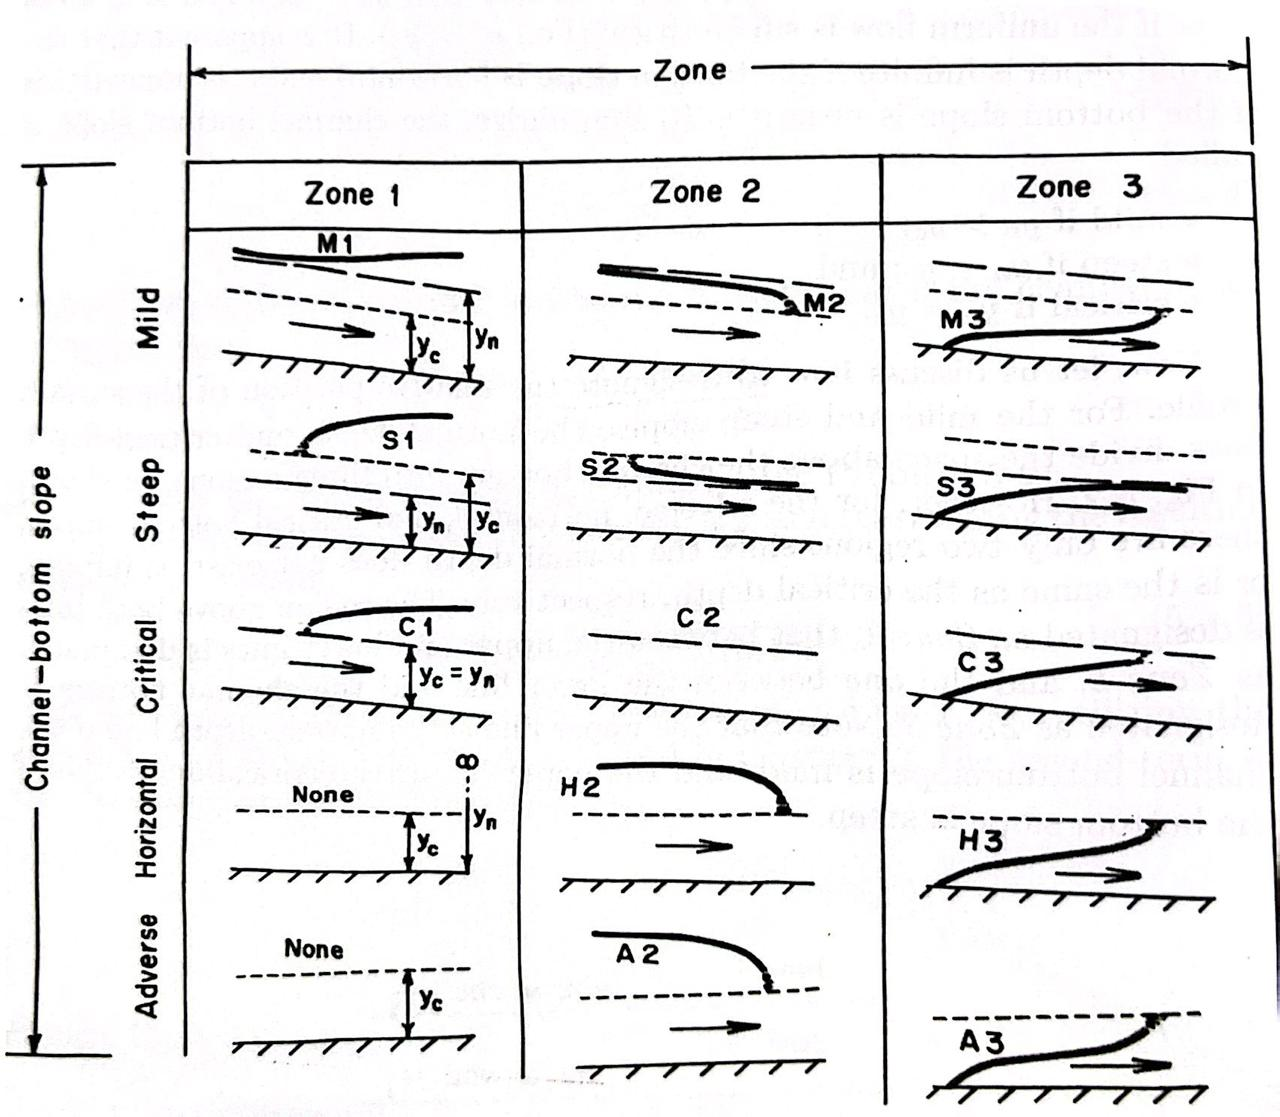
\includegraphics[width=8cm]{fig53.jpeg}
\caption{Perfiles de la l\'amina de flujo (tomado de \cite{Chau}).}
\label{fig3}
\end{figure}
 
El comportamiento de los  perfiles de l\'amina de agua se puede hacer con base en el an\'alisis de la ecuaci\'on~\ref{eq5}. De acuerdo con esto, $y$ aumentar\'a a lo largo de $x$ si $\frac{dy}{dx}$ es positivo y decrecer\'a si ocurre lo contrario. El signo de $\frac{dy}{dx}$ lo determina la parte derecha de la ecuaci\'on~\ref{eq5}; los signos del numerador ($S_o - S_f $) y del denominador ($1-F_r^2$). Del estudio de flujo uniformes sabemos que $S_f = S_o = S_w$ cuando $y_n = y$, por lo que para un $Q$ dado a partir de la ecuaci\'on de Manning o de Chezy tenemos que $S_f > S_o$ si $y< y_n$ y $S_f < S_o$ si $y > y_n$. De acuerdo con esto, podemos establecer el signo de $S_o - S_f$. El signo de ($1-F_r^2$) se determina si el flujo es subcritico ($F_r < 1$) o supercritico ($F_r > 1$). 

Ahora miremos como la superficie de la l\'amina de agua se aproxima a la profundidad normal, a la profundidad cr\'itica o al fondo del canal. Si $y \rightarrow y_n$ entonce $S_f \rightarrow S_o$ y por lo tanto $\frac{dy}{dx} \rightarrow 0$ a pesar que $Fr \neq 1$ (no flujo cr\'itico). Esto significa que  la l\'amina de agua se aproxima asint\'oticamente a $NDL$. Por otro lado, si $y \rightarrow y_c$ $F_r \rightarrow 1$ por que el denominador tiende a cero. Esto quiere decir que $\frac{dy}{dx} \rightarrow \infty$ a pesar que $S_f \neq S_o$. Esto significa que la l\'amina de agua se aproxima a $CDL$ verticalmente. En realidad no se aproxima verticalmente ya que esto no es posible f\'isicamente, pero si con una pendiente muy alta. A pesar que te\'oricamente la l\'amina de agua se aproxima verticalmente esto no es posible ya que las distribuciones de presiones cuando la  l\'amina de agua se curva fuertemente la presi\'on ya no es hidroest\'atica por lo tanto la ecuaci\'on~\ref{eq5} se viola.  

Por otro lado, cuando $y \rightarrow \infty$, $V \rightarrow 0$ y por lo tanto $F_r$ y $S_f$ tienden a cero. De la ecuacion~\ref{eq5}, tenemos entonces que $\frac{dy}{dx} \rightarrow S_o$. Teniendo en cuenta que para FGV se asume una pendiente pequeña, tenemos que $\frac{dy}{dx} \approx 0$ por lo que la l\'amina de agua tiende  a ser horizontal. 

Analicemos ahora lo que ocurre cuando la l\'amina de agua se aproxima al fondo del canal (e.g $y \rightarrow$). De la ecuaci\'on de Chezy, tenemos que:

$$
S_f = \frac{Q^2}{C^2 A^2 R}
$$

donde $C$ es la constante de Chezy, $R= A/P$ es el radio hidr\'aulico. Note que para un canal rectangular muy ancho de ancho $B$, se tiene que $R \approx y$. Reemplazando en la ecuaci\'on~\ref{eq5}, tenemos que:
$$
\frac{dy}{dx} = \frac{gB \left(S_o C^2 B^2 y^3 - Q^2\right)}{C^2 \left(gBy^3 -\alpha B Q^2\right)}
$$

Teniendo en cuenta que $y\rightarrow 0$ cuando se aproxima al fondo del canal, la ecuaci\'on anterior se convierte en:
$$
\lim_{y \to 0} \frac{dy}{dx} = \frac{g}{\alpha C^2}
$$
Lo anterior quiere decir que cuando $y \rightarrow 0$, la pendiente de la l\'amina de agua $dy/dx$ es finita, tiene un valor positivo y es una funci\'on de $C$ y de $\alpha$. Sin embargo, si se usa la ecuaci\'on de Manning en lugar de la ecuaci\'on de Chezy, se tiene que $\frac{dy}{dx} \rightarrow \frac{0}{0} \rightarrow \infty$ si $y \rightarrow 0$.

Con base en lo anterior, analisemos los perfiles de l\'amina de agua cuando $S_o$ es suave, esto quiere decir que $y_n > y_c$. Si analizamos la profundidad de la l\'amina de agua en las tres zonas:
\begin{itemize}
    \item Zona 1: $y > y_n > y_c$
    \item Zona 2: $y_n > y > y_c$
    \item Zona 2: $y_n > y_c > y$
\end{itemize}

\subsubsection*{Zona 1 (perfil M1)}
Si $y > y_n$, de la ecuaci\'on de Manning o Chezy, se tiene que $S_f < S_o$ lo que significa que el numerador es positivo  en la ecuaci\'on~\ref{eq5}. Como $y > y_c$, $F_r < 1$ por lo que el denominador de la ecuaci\'on~\ref{eq5} es positivo. Los s\'ignos de la ecuacion\ref{eq5} son:
$$
\frac{dy}{dx} = \frac{S_o - S_f}{1-F_r^2} = \frac{+}{+} = +
$$
Lo anterior significa que $y$ se incrementa a lo largo de $x$; crece hacia aguas abajo. Cuando $y \rightarrow y_n$ asint\'oticamente en direcci\'on aguas arriba ($S_f \rightarrow S_o$), la superficie del agua tiende a ser horizontal ($\frac{dy}{dx}\rightarrow 0$).  

\subsubsection*{Zona 2 (perfil M2)}
Si $y < y_n$, de la ecuaci\'on de Manning o Chezy, se tiene que $S_f > S_o$. Esto quiere decir que el numerador en la ecuaci\'on~\ref{eq5}, es negativo. El denominador sigue siendo positivo porque $F_r < 1$ y $y > y_c$. Los s\'ignos de la ecuaci\'on~\ref{eq5} quedan:
$$
\frac{dy}{dx} = \frac{S_o - S_f}{1-F_r^2} = \frac{-}{+} = -
$$
Esto quiere decir que $y$ decrece a lo largo de $x$; hacia aguas abajo en donde $y \rightarrow y_c$ asint\'oticamente y c\'asi vertical. Hacias aguas arriba, $y \rightarrow y_n$ asint\'oticamente.

\subsubsection*{Zona 3 (perfil M3)}
Si $y < y_n$, de la ecuaci\'on de Manning o de Chezy, se tiene que $S_f > S_o$, lo cual significa que el numerador de la ecuaci\'on~\ref{eq5} es negativo. Como $y < y_c$, $F_r >1$ por lo que el denominador de la ecuaci\'on~\ref{eq5} es negativo. Los s\'ignos de la ecuaci\'on~\ref{eq5}, son:
$$
\frac{dy}{dx} = \frac{S_o - S_f}{1-F_r^2} = \frac{-}{-} = +
$$
Esto significa que $y$ incrementa a lo largo de $x$; en direcci\'on aguas abajo. Hacia aguas abajo donde $y \rightarrow y_c$ c\'asi verticalmente, mientras que en direcci\'on aguas arriba cuando $y \rightarrow 0$ la pendiente de la l\'amina de agua es finita y positiva (de acuerdo con la ecuaci\'on de Chezy). 

La figura~\ref{fig4} muestra los perfiles de flujo en situaciones reales.
% Chau fig 5.4
\begin{figure}[h]
\centering
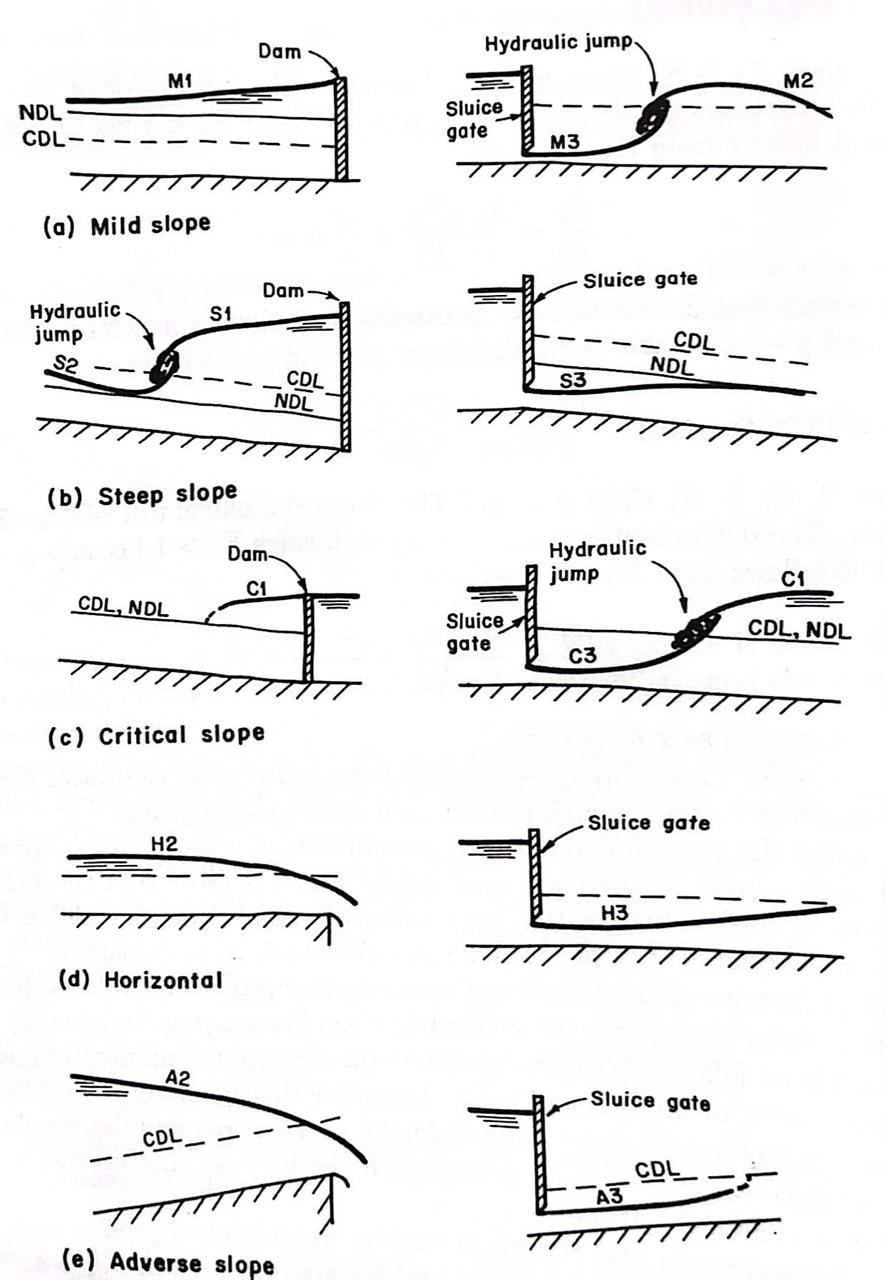
\includegraphics[width=8cm]{fig54.jpeg}
\caption{Perfiles de la l\'amina de agua (tomado de \cite{Chau}).}
\label{fig4}
\end{figure}

\subsection{¿Como esquematizar los perfiles de flujo?}
Es importante anotar que una secci\'on de flujo en donde exista una relaci\'on entre $Q$ y $y$ (e.g. $f(y)=Q$) es una \emph{secci\'on de control}. El comportamiento de los perfiles de flujo analisados son para canales prism\'aticos con secciones de control aguas arriba o aguas abajo. Sin embargo, en la vida real, los controles sobre el flujo pueden existir en cualquier secci\'on a lo largo del flujo y la geometr\'ia asi como la pendiente pueden cambiar a lo largo del canal por lo que la esquematizaci\'on de los perfiles se debe hacer por sectores del canal. A continuaci\'on describe como esquematizar el perfil de flujo en canal:
\begin{enumerate}
    \item Divida el canal en diferentes tramos con una \'unica geometr\'ia, pediente, caudal y coeficiente de fricci\'on.
    \item Calcule la profundidad normal ($y_n$) y la profundidad cr\'itica ($y_c$).
    \item Para cada tramo, dibuje el fondo del canal, la l\'inea de $y_n$ y de $y_c$.
    \item Determine las secciones de control, aquellas secciones en donde $y$ es conocida e.g. secciones en donde $y = y_c$. Indentifique los tramos en donde el flujo es uniforme $y = y_n$.
\end{enumerate}
Note que el flujo subcr\'itico es gobernado por  secciones de control aguas abajo, mientras que el flujo supercr\'itico es gobernado por secciones de control aguas arriba. Es posible tener secciones de control intermedias como vertederos, compuertas, etc, que determinan el flujo aguas arriba y aguas abajo. Por ejemplo, a la entrada de un canal, la profundidad de flujo pasa a trav\'ez de $y_c$ cuando el nivel en el tanque o vertedero es mayor que $y_c$ y la pendiente del canal es alta. En un canal que descarga libremente, si $y > y_c$, la l\'amina de agua pasa por $y_c$ aproximadamente de 3 a 4 veces $y_c$ aguas arriba de la secci\'on de descarga. Por otra parte, un resalto hidr\'aulico es formado cuando se presenta un cambio de flujo supercr\'itico a subcr\'itico; en este caso se tiene un control aguas arriba y otro aguas abajo del resalto.

% Ej 5.1 Chau 
\begin{eje}{}{eje1}
Esquematice el perfil de flujo de el canal que conecta los tanques que muestra la figura. Tenga en cuenta que la pendiente del canal 1 es fuerte y la pendiende del canal 2 es suave.
%\centering
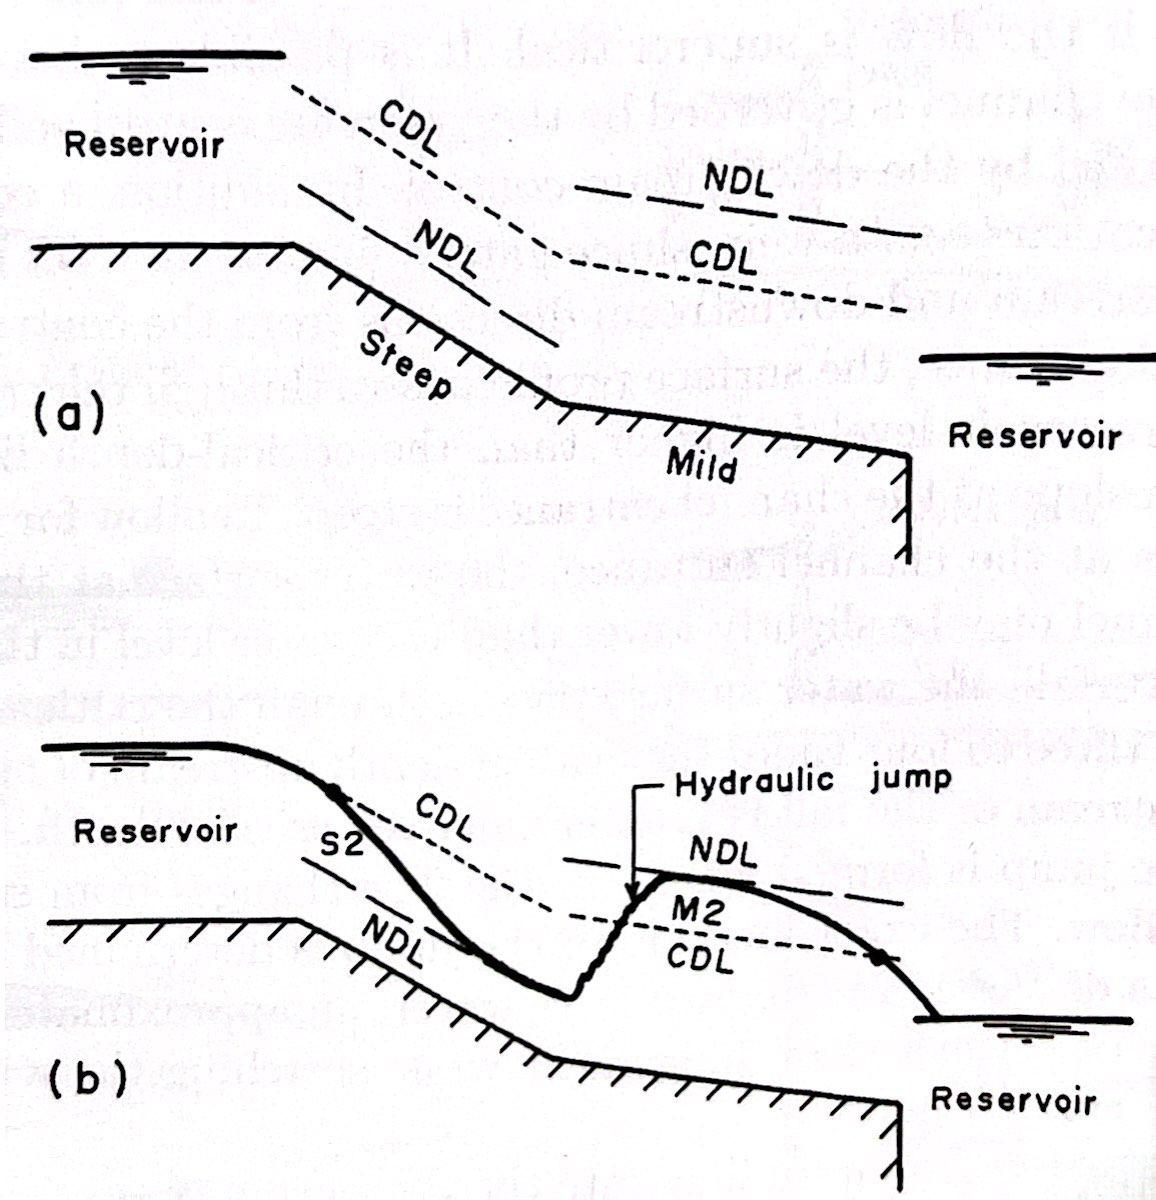
\includegraphics[width=8cm]{fig51e.jpeg}
\end{eje}

\subsection{Casos t\'ipicos relacionados con perfiles de flujo}
\subsubsection*{Descarga de un embalse}
Consideremos el sistema mostrado en la figura~\ref{fig6} en donde un embalse descarga hacia un canal en donde la secci\'on transversal, el coeficiente de p\'erdidas de energ\'ia a la entrada ($k$), el coeficiente de rugosidad de Manning ($n$) y la pendiente del fondo del canal $S_o$, son conocidas. El problema consiste en determinar la profundidad de la l\'amina de agua ($y$) y el caudal de flujo ($Q$). Note que como el embalse es grande, la velocidad de flujo justo antes de la entrada al canal es cero y el nivel de la l\'amina de agua ($H_o$) es constante y conocido.  

% Chau fig 5.8
\begin{figure}[h]
\centering
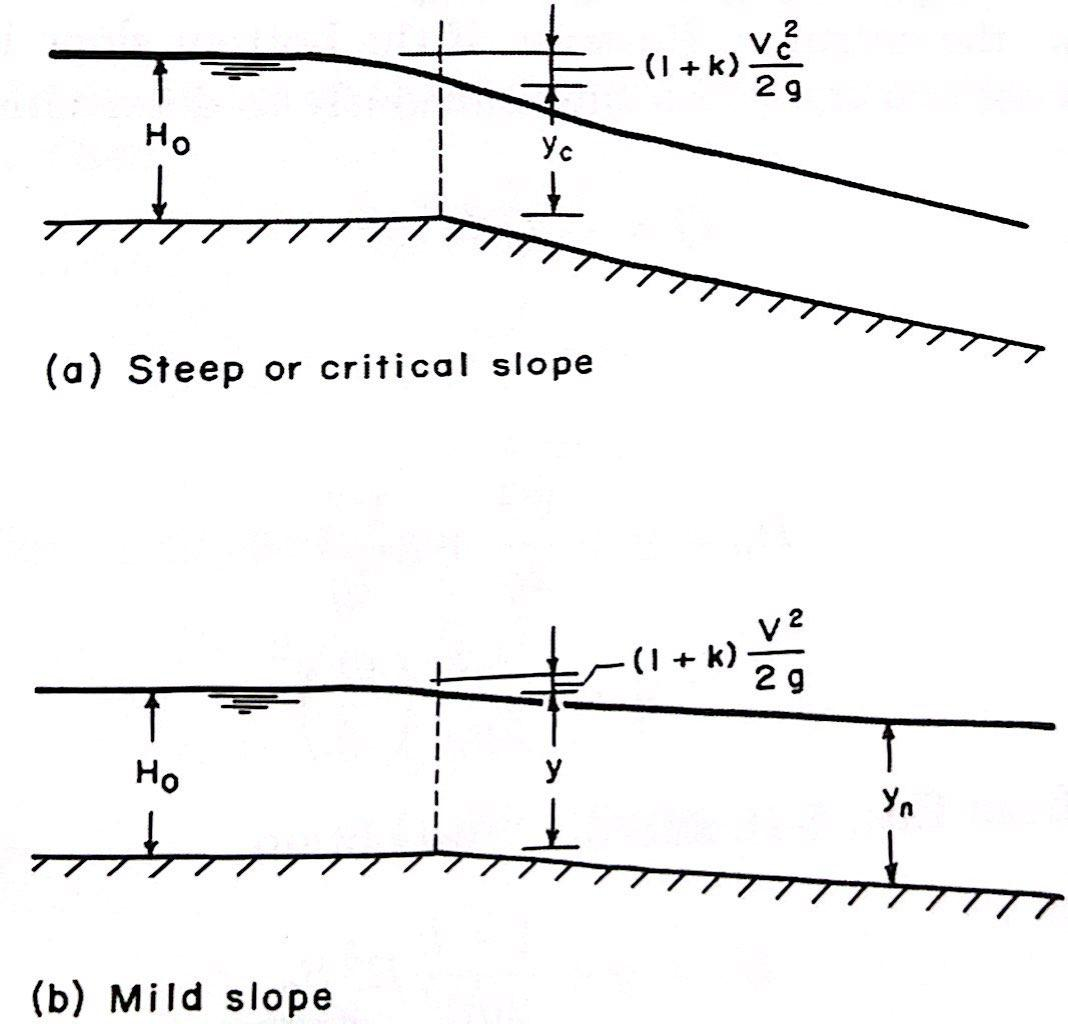
\includegraphics[width=8cm]{fig58.jpeg}
\caption{Descarga desde un embalse (tomado de \cite{Chau}).}
\label{fig6}
\end{figure}

Como  $S_o$ puede ser suave, cr\'itica o fuerte, tenemos que la posici\'on de $CDL$ y $NDL$ cambia. Si $S_o$ es fuerte o cr\'itica, $y$ cortar\'a  $CDL$ justo a la entrada del canal y seguir\'a disminuyendo hasta encontrar una profundidad uniforme $y<y_c$ para el caso de pendiente fuerte y $y = y_c$ para el caso de pendiente cr\'itica. Si $S_o$ es suave, $y$ se aproximadara a $NDL$ r\'apidamente justo aguas abajo de la entrada.

El primer paso, es determinar el tipo $S_o$. Para esto se calcula la pendiente cr\'itica del canal $S_c$. Si consideramos que $y_c$ ocurre a la entrada del canal, para un $\alpha$, tenemos que:

$$
\frac{Q^2}{2g A_c^2} = \frac{D_c}{2}
$$
y 
$$
H_o = y_c + (1 + k) \frac{Q^2}{2g A_c^2}
$$
donde $k$ es el coeficiente de p\'erdidas a la entrada, y $D_c$ y $A_c$ son la profundidad hidr\'aulica y el \'area mojada, respectivamente, para $y_c$. Estas dos ecuaciones son resueltas para $Q$ y $y_c$. Si la pendiente del fondo del canal es igual a $S_c$, tendr\'iamos un flujo uniforme ($y = y_n = y_c$) a partir de la entrada al canal y podr\'iamos utilizar la ecuaci\'on de Manning para encontrar $S_c$:

$$
Q = \frac{1}{n}A R^{2/3} S_c^{1/2}
$$

Una vez calculada $S_c$ a partir de la ecuaci\'on anterior, podemos decir que la pendiente es cr\'itica si $S_o = S_c$, la pendiente es fuerte si $S_o > S_c$ y la pendiente es suave si $S_o < S_c$. Si $S_o = S_c$ $Q$ y $y = y_n = y_c$, calculadas a partir de las ecuaciones, son correctas. Si $S_o > S_c$ solo el caudal es correcto y la profundidad $y = y_n$ se calcula a partir de la ecuaci\'on de Manning. Si $S_o < S_c$ ni $Q$ ni $y$ est\'an bien calculadas y es necesario resolver las siguientes ecuaciones para encontrarlas:

$$
Q = \frac{1}{n}A R^{2/3} S_o^{1/2}
$$

y 

$$
H_o = y + (1 + k) \frac{Q^2}{2gA^2}
$$

Uniendo estas dos ecuaciones, tenemos que:
$$
H_o = y + \frac{1 + k}{2g n^2} R^{4/3} S_o
$$

Resolviendo esta ecuaci\'on encontramos $y$ en el canal, y $Q$ se puede encontrar utilizando la ecuaci\'on de Manning. 

% Ej 5.3 Chau 
\begin{eje}{}{eje3}
Un canal rectangular en concreto ($n = 0.013$) de $B = 10$ m de ancho que tiene una pendiente del fondo $S_o = 0.01$ sirve para descargar un embalse de nivel constante. Si el nivel en el embalse es de $H_o = 6$ m, determinar el caudal y la profundidad teniendo en cuenta que la velocidad en el embalse es cero y las p\'erdidas a la entrada del canal son despreciables.      
\end{eje}


\subsection{Perfiles de flujo en canales compuestos}
El c\'alculo de perfiles de flujo mostrado hasta el momento ha sido para canales con secciones \'unicas. Sin embargo, en canales con secciones compuestas (canales con bancas o diferentes rugosidades) los perfiles de flujo necesitan un tratamiento especial porque puede haber m\'as de una profundidad cr\'itica. Para el an\'alisis de estos perfiles de flujo es importante dibujar las curvas de energ\'ia y fuerza espec\'ifica y determinar las profundidades cr\'iticas. El siguiente ejemplo muestra como determinar el perfil de flujo para una canal compuesto. 

% Ej 5.4 Chau 
\begin{eje}{}{eje4}
Un canal largo de secci\'on transversal como se muestra en la figura, descarga libremente a un embalse. El canal transporta un caudal constante de $Q = 2.5$ m$^3$s$^{-1}$ y los coeficientes de rugosidad para el canal principal y las bancas son de 0.013 y 0.0144, respectivamente (ver figura). Esquematizar los perfiles de velocidad si el fondo del canal tuvier\'a las siguientes pendientes: $S_o = 0.0094$, $S_o = 0.0049$, $S_o = 0.0029$ y $S_o = 0.001$.  
%\centering
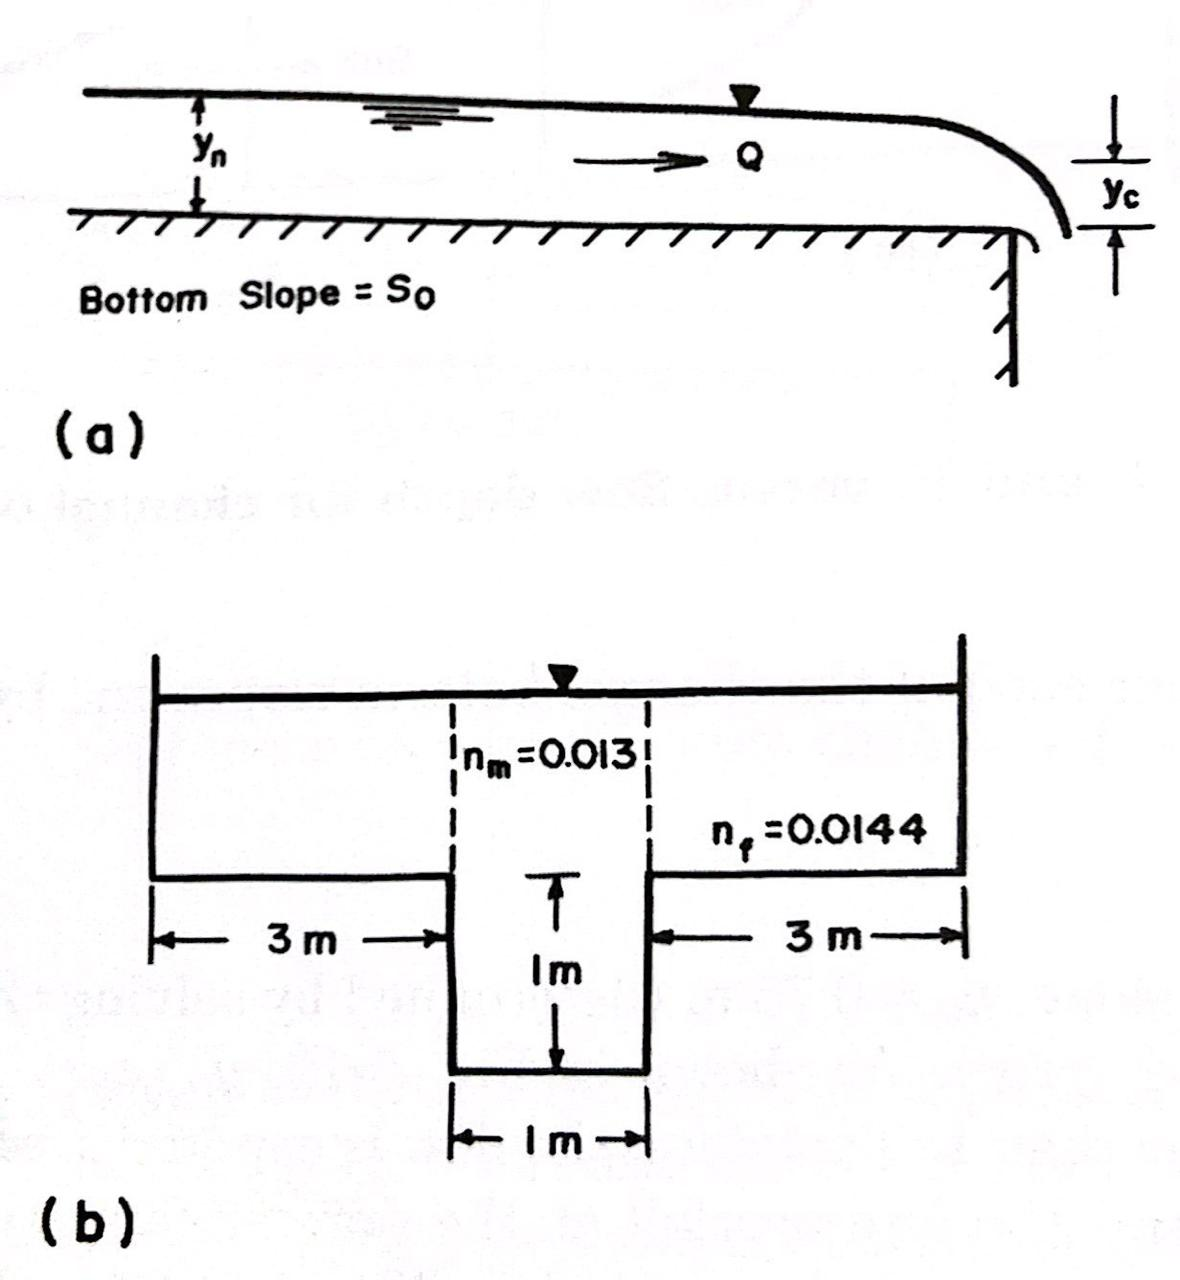
\includegraphics[width=8cm]{fig54e.jpeg}
\end{eje}


\subsection{C\'alculo del flujo gradualmente variado}
En ingenier\'ia hidr\'aulica, es necesario, en muchos casos, determinar el perfil de la l\'amina de agua a lo largo de un canal para un caudal determinado. Este c\'alculo es importante para la planeaci\'on, diseño y operaci\'on de canales, y para evaluar los efectos en la hidr\'aulica del canal para diferentes modificaciones. Por ejemplo, la construcci\'on de una presa en un r\'io, modifica el perfil de la l\'amina de agua aguas arriba por lo que es necesario calcularlo para determinar el \'area inundada. El c\'alculo del flujo gradualmente variado (FGV) consiste en determinar la profundidad y la velocidad en cada secci\'on del canal a partir de las ecuaciones de conservaci\'on de la masa, conservaci\'on de la energ\'ia y conservaci\'on de la cantidad de movimiento lineal, para un $n$ de Manning, $S_o$, $Q$ y geometr\'ia de la secci\'on, usualmente, conocidas. Como comentabamos en secciones anteriores, el cambio en la profundidad de flujo en FGV es pequeño por lo que se puede asumir una distribuci\'on hidroest\'atica de presiones.  

Para determinar el perfil de la l\'amina de agua a lo largo del canal, es necesario solucionar la ecuaci\'on~\ref{eq4}, la cual es una ecuaci\'on diferencial ordinaria de primer orden en donde $x$, que es la longitud en direcci\'on del flujo, es la variable independiente y $y$, que es la profundidad del flujo, es la variable dependiente. Note que la ecuaci\'on~\ref{eq4} es funci\'on de $x$ y de $y$, ya que la geometr\'ia, $n$, $S_o$ y $Q$ son valores dados. De acuerdo con esto es posible escribir:

\begin{equation}
    \frac{dy}{dx} = f(x,y)
\label{eq6}
\end{equation}

por lo que

\begin{equation}
    f(x,y) = \frac{S_o - S_f }{1-\left(\alpha B Q^2 \right) /\left(g A^3 \right)}
\label{eq7}
\end{equation}

La ecuaci\'on~\ref{eq7}, la cual es una ecuaci\'on no lineal,  se soluciona por integraci\'on num\'erica teniendo en cuenta que su soluci\'on anal\'itica no es posible para el caso general. Esta soluci\'on num\'erica se hace para valores discretos de $x$ para los cuales se determina el valor de $y$ partiendo de un valor inicial $y$ conocido para $x$. Supongamos que $y_1$ es un valor conocido en $x_1$ y se quiere conocer $y_2$ para $x_2$ o $x_2$ para $y_2$. Esto implica dos tipos de problemas: 1) calcular $y_2$ para $x_2$ y 2) conocer $x_2$ si se conoce $y_2$. Despejando e integrado la ecuaci\'on~\ref{eq6}, se tiene:

\begin{equation}
    \int_{y_1}^{y_2} dy = \int_{x_1}^{x_2} f(x,y) dx
\label{eq8}
\end{equation}

Resolviendo, se tiene:

\begin{equation}
    y_2 = y_1 +  \int_{x_1}^{x_2} f(x,y) dx
\label{eq9}
\end{equation}

La ecuaci\'on~\ref{eq9} sirve para econtrar de manera secuencial los valores de $y$ aguas abajo en direcci\'on $x$ positiva a partir de un valor $y_1$ y de $f(x,y)$ en $x_1$ conocidos. De igual manera es posible encontrar los valores de $y$ aguas arriba en direcci\'i'on de $x$ negativa partiendo de un valor dado de $y_2$ y de $f(x,y)$ en $x_2$ conocidos.

Para el problema dos, el cual consiste en encontrar $x_2$ si se conoce $y_2$, a partir de la ecuaci\'on~\ref{eq6} tenemos:

\begin{equation}
    \frac{dx}{dy} = f^{-1}(x,y)
\label{eq10}
\end{equation}

Despejando e integrando:

\begin{equation}
    x_2 = x_1 + \int_{y_1}^{y_2}  f^{-1}(x,y) dy
\label{eq11}
\end{equation}

La ecuaci\'on~\ref{eq11} sirve para econtrar de manera secuencial los valores de $x$ aguas abajo en direcci\'on $x$ positiva a partir de un valor $x_1$ y de $f(x,y)$ en $x_1$ conocidos. De igual manera, es posible encontrar los valores de $x$ aguas arriba en direcci\'i'on de $x$ negativa partiendo de un valor dado de $x_2$ y de $f(x,y)$ en $x_2$ conocidos.

Como una alternativa a la soluci\'on de la ecuaci\'on~\ref{eq4}, es la soluci\'on de la ecuaci\'on de conservaci\'on de la energ\'ia entre dos secciones adyacentes 1 y 2,

\begin{equation}
    z_1 + y_1 + \alpha_1 \frac{V_1^2}{2g} = z_2 + y_2 + \alpha_2 \frac{V_2^2}{2g}  + h_f
\label{eq12}
\end{equation}

donde $h_f$ es la p\'erdida de energ\'ia entre 1 y 2. Esta ecuaci\'on algebr\'aica se soluciona para la secci\'on 1 o 2 dependiendo en cual de ellas sean conocidas las condiciones de flujo. Note que $h_f$ se calcula a partir de la ecuaci\'on de Manning, por ejemplo. Note que todo lo que debemos saber para solucionar la ecuaci\'on~\ref{eq4} o la ecuaci\'on~\ref{eq12} son las condiciones del flujo  en una secci\'on (secci\'on de control) e ir calculando hacia aguas arriba o hacia aguas abajo dependiendo del tipo de problema, las propiedades del flujo (e.g. $y$). Un aspecto importante a tener en cuenta es el  paso en $x$ con el fin de que la soluci\'on num\'erica sea estable.  

%Note que el calculo inicia a partir de una secci\'on en donde las condiciones de flujo son conocidas. Deciamos anteriormente que la secci\'on de control del flujo subcritico estaba aguas abajo mientras que las secci\'on de control del flujo supercritico estaba aguas arriba. 

En las siguientes secciones se explican algunos m\'etodos para el c\'alculo del flujo gradualmente variado. El c\'alculo del perfil en los dos primeros m\'etodos se hace secci\'on a secci\'on. Se introducen ademas m\'etodos num\'ericos m\'as sofisticados para el c\'alculo del FGV.  

\subsubsection{M\'etodo del paso directo}
Este m\'etodo es un procedimiento sistem\'atico para determinar la posici\'on $x_2$ en donde ocurre una profundidad conocida $y_2$ a partir de las condiciones conocidas en una secci\'on 1 ($x_1$ y $y_1$) para un $Q$, $S_o$ y $n$ conocidos (ver figura~\ref{fig8}).
% Chau fig 6.2
\begin{figure}[h]
\centering
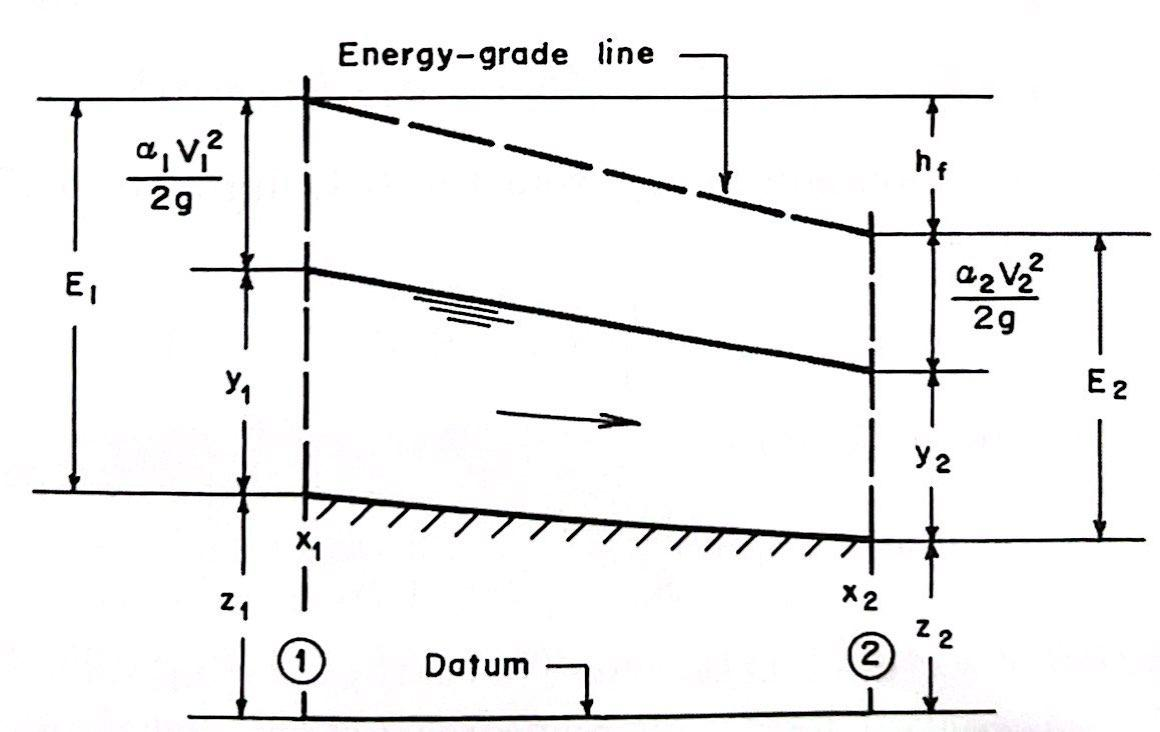
\includegraphics[width=8cm]{fig62.jpeg}
\caption{C\'alculo de la distancia para un profundidad conocida (tomado de \cite{Chau}).}
\label{fig8}
\end{figure}

Partiendo de la ecuaci\'on de conservaci\'on de la energ\'ia (ecuaci\'on~\ref{eq12}) entre dos secciones 1 y 2, tenemos que:
\begin{equation}
    z_1 + E_1 = z_2 + E_2  + h_f
\label{eq13}
\end{equation}

en donde $E_i = y_i + \alpha_i \frac{V_i^2}{2g}$. Las p\'erdidas de energ\'ia $h_f$ entre 1 y 2, se pueden calcular como:
$$
h_f = \frac{1}{2}\left( S_{f_1} + S_{f_2} \right)  (x_2 - x_1)
$$
en donde $S_{f_i}$ puede ser calculada usando una de las ecuaciones para el c\'alculo de p\'erdidas en flujo uniforme como la ecuaci\'on de Manning. La ecuaci\'on~\ref{eq13} queda:

\begin{equation}
    z_1 + E_1 = z_2 + E_2  + \frac{1}{2}\left( S_{f_1} + S_{f_2} \right)  (x_2 - x_1)
\label{eq14}
\end{equation}

De la figura~\ref{fig8} tenemos que $z_2 = z_1 - S_o \left( x_2 - x_1 \right)$, reemplazando en la ecuaci\'on~\ref{eq14} y despejando para $x_2$:

\begin{equation}
    x_2 = x_1 + \frac{E_2 - E_1}{S_o - \frac{1}{2}\left( S_{f_1} + S_{f_2} \right)}
\label{eq15}
\end{equation}

La ecuaci\'on~\ref{eq15} determina la localizaci\'on $x$ de la secci\'on 2 a partir de unos valores dados de $Q$, $S_o$ y $n$, a partir de condiciones conocidas de flujo en la secci\'on 1, y a partir de unos valores dados de $y_2$ para calcular $E_2$. A partir de la secci\'on conocida 1, se inicia el c\'alculo sistem\'atico de $x$ para valores dados de $y$ aguas abajo ($x$ positivo) o hacia aguas arriba ($x$ negativo) dependiendo de donde se encuentre la secci\'on inicial. Note que el signo del c\'alculo es tenido en cuenta en la ecuaci\'on~\ref{eq15}. Para el c\'alculo es importante utilizar el mayor n\'umero de cifras significat\'ivas teniendo en cuenta que el segundo t\'ermino del lado derecho de la ecuaci\'on~\ref{eq15} es muy pequeño. Algunas desventajas de este m\'etodo son: 1) no c\'alculo de la profundidad de agua $y$ por lo que ser\'ia necesario interpolar para saber $y$ en una posici\'on  determinada, 2) en canales con geometr\'ia variable ser\'ia necesario determinar la geometr\'ia mediante un proceso iterat\'ivo ya que esta no se conoce en 2. 

A continuaci\'on se describe un algoritmo para la implementaci\'on del m\'etodo de paso directo.
\begin{alg}{C\'alculo del FVG en canales prism\'aticos o circulares: M\'etodo del paso directo}{alg1}
\begin{enumerate}
\item Leer: $Q$, $n$, $So$, $\alpha$, $y_1$ y $x_1$, donde $y_1$ es la profundida de flujo en la secci\'on de control y $x_1$ es la abscisa de la secci\'on de control.  En caso de canales prism\'aticos leer: $b$, $\theta_1$ (\'angulo de la banca izquierda) y $\theta_2$ (\'angulo de la banca izquierda). En el caso de secciones circulares, leer $r$ (radio). Note que en caso de que en la secci\'on de control la profundidad $y_1 = y_c$, el valor de $y_1$ no se lee; se har\'a igual a $y_c$ una ves sea calculada.   
\item Calcular la profundidad normal ($y_n$) usando la ecuaci\'on de Manning y la profundidad cr\'itica ($y_c$) usando la ecuaci\'on de n\'umero de Froude. 
\item Con base en $y_n$, $y_c$ y $So$ determinarl el tipo de perfil de flujo.
\item Establecer si la secci\'on de control de flujo esta aguas arriba o aguas abajo. 
\item Leer $\Delta y$, el cual es el paso para aumetar o disminuir (dependiendo del perfil) la profundidad. $\Delta y$ se establece como la diferencia entre $y_1$ y la profundidad que alcanzar\'a el perfil de flujo hacia aguas arriba o hacia aguas abajo, puede ser $y_n$ o $y_c$. Note que $\Delta y$ debe asegurar que existan un n\'umero suficiente de puntos para graficar el perfil. 
\item Elaborar una tabla con las siguientes columnas: $y$ (profundidad de flujo), $A$ (\'Area), $R$ (Radio hidr\'aulico), $V$ (Velocidad de flujo), $S_f$ (gradiente de energ\'ia) y $E$ (Energ\'ia). La primera fila de la tabla se calcula con los valores conocidos en la secci\'on de control $1$. Para la segunda fila (la secci\'on siguiente $2$),  la profundidad $y_1$ se disminuye o se aumenta (dependiendo del tipo de perfil) en un valor $\Delta y$, $y_2 = y_1 \pm \Delta y $. A partir de $y_2$ se calculan los valores de la tabla para completar la fila 1. 
\item A partir de los valores calculados en la tabla para la fila $i$ y la fila $i+1$, se calcula la abscisa $x_{i+1}$ usando la ecuaci\'on~\ref{eq15}. El c\'alculo de los valores de $x$ se hace hasta que:
    \begin{itemize}
        \item $y>=1.05 y_n$ en caso de que $y$ disminuya y se aproxime a $y_n$.
        \item $y<=0.98 y_n$ en caso de que $y$ aumente y se aproxime a $y_n$.
        \item $y>=1.05 y_c$ en caso de que $y$ disminuya y se aproxime a $y_c$.
        \item $y<=0.98 y_c$ en caso de que $y$ aumente y se aproxime a $y_c$.
    \end{itemize}

\item Con las parejas de valores ($x$, $y$) graficar el perfil de flujo. Otras parejas de puntos utiles para graficar son: ($x$, $z$), ($x$, $y_n$) y ($x$, $y_c$). En las dos ultimas los valores de $y_n$ y $y_c$ se repiten. Note que $z_{i+1} = z_{i+1} + So \left( x_{i+1} - x_i \right)$

\end{enumerate}
\end{alg}

% Ej 6.1 Chau 
\begin{eje}{}{eje5}
 Para una canal trapezoidal con las siguientes caracter\'isticas:
 \begin{itemize}
     \item Pendiente de fondo $So =$ 0.001
     \item Caudal $Q = $ 30 m$^3$ s$^{-1}$
     \item Ancho de base $b =$ 10 m
     \item Coeficiente de rugosidad de Manning $n = $ 0.013
     \item Profundidad en la secci\'on de control aguas abajo $y_1 = $ 5 m en $x_1 =$ 0 m.
     \item $\alpha = $1
 \end{itemize}
 calcular el perfil de la l\'amina de agua utilizando el m\'etodo del paso directo. 
\end{eje}




\subsubsection{M\'etodo del paso estandard}
El m\'etodo del paso directo no es adecuado si queremos determinar la profundidad en un secci\'on determinada o si el canal tiene una geometria irregular como es el caso de canales naturales. El \emph{m\'etodo del paso estandard} aparece como el procedimiento m\'as adecuado para el c\'alculo de perfiles de flujo en cualquier tipo de canales. Este m\'etodo es el implementado dentro del programa  HEC-RAS, el cual es un c\'odigo de uso libre muy popular desarrollado por el U.S. Army Corps of Engineers. 

Al observar la figura~\ref{fig9}, se desea calcular la profundidad $y_2$ en una seccion $x_2$ a partir de un caudal Q, una pendiente $So$, una rugosidad de Manning $n$ y una geometr\'ia conocidas en un tramo de canal incluyendo, una profundidad conocida  $y_1$ en $x_1$.

% Chau fig 6.3
\begin{figure}[h]
\centering
\includegraphics[width=8cm]{fig63.jpeg}
\caption{C\'alculo de la profundidad de flujo en una secci\'on determinada (tomado de \cite{Chau}).}
\label{fig9}
\end{figure}

Partiendo de la profundidad $y_1$ y de $Q$ se puede calcular la $V_1$ a trav\'es de $V_1=Q/A_1$, donde $A_1$ es la secci\'on transversal en 1. Se puede entonces calcular la energ\'ia total en 1 $H_1$ como:

\begin{equation}
    H_1 = z_1 + y_1 + \alpha_1 \frac{V_1^2}{2g}
\label{eq16}
\end{equation}

y por lo tanto, la energ\'ia total en 2 $H_2$ es:
\begin{equation}
    H_2 = H_1 - h_f
\label{eq17}
\end{equation}
donde $h_f$ son las perdidas de energ\'ia entre las secciones 1 y 2. La ecuaci\'on~\ref{eq17}, en funci\'on del gradiente de energ\'ia, se puede expresar como:
\begin{equation}
    H_2 = H_1 - \frac{1}{2}\left( S_{f_1} + S_{f_2} \right)\left( x_2 - x_1 \right)
\label{eq18}
\end{equation}
Reemplazando por los terminos de la energ\'ia total para $H_2$ en la ecuaci\'on~\ref{eq18} y re-organizando se tiene:
\begin{equation}
y_2 + \frac{\alpha_2 Q^2}{2g A_2^2} + \frac{1}{2}S_{f_2} \left( x_2 - x_1 \right) + z_2 - H_1 + \frac{1}{2}S_{f_1}\left( x_2 - x_1 \right) = 0
\label{eq19}
\end{equation}

En la ecuaci\'on~\ref{eq19}, $A_2$ y $S_{f_2}$ son funciones de la variable desconocida $y_2$. Los otros t\'erminos son dados o han sido calculados para la secci\'on 1. De acuerdo con esto, $y_2$ es econtrado tras solucionar la ecuaci\'on no linear:
\begin{equation}
f\left( y_2 \right) = y_2 + \frac{\alpha_2 Q^2}{2g A_2^2} + \frac{1}{2}S_{f_2} \left( x_2 - x_1 \right) + z_2 - H_1 + \frac{1}{2}S_{f_1}\left( x_2 - x_1 \right)
\label{eq20}
\end{equation}

La ecuaci\'on~\ref puede ser resuelta por medio de el \emph{m\'etodo de Newton-Raphson} o el \emph{m\'etodo de la bisecci\'on}. A continuaci\'on se discutir\'a el m\'etodo de Newton-Raphson para resolver la ecuaci\'on~\ref{eq20} y para esto es necesario el c\'alculo de la derivada de $f\left( y_2 \right)$ con respecto a $y_2$ como:
\begin{equation}
    \frac{df}{y_2} = 1 - \frac{\alpha_2 Q^2}{g A_2^3}\frac{dA_2}{dy_2} + \frac{1}{2}\left( x_2 - x_1 \right)\frac{d}{dy_2}\left( \frac{Q^2 n^2}{C_o^2 A_2^2 R_2^{4/3}} \right)
\label{eq21}
\end{equation}
Resolviendo la derivada de el \'ultimo termino de la ecuaci\'on~\ref{eq21}, se tiene:

\begin{equation}
\begin{split}
    \frac{d f}{dy_2}\left( \frac{Q^2 n^2}{C_o^2 A_2^2 R_2^{4/3}} \right) &= \frac{-2 Q^2 n^2}{C_o^2 A_2^3 R_2^{4/3}}\frac{d A^2}{dy_2} - \frac{4}{3}\frac{Q^2 n^2}{C_o^2 A_2^3 R_2^{4/3}}\frac{1}{R_2}\frac{d R_2}{dy_2} \\
                                                                       &= \frac{-2 Q^2 n^2}{C_o^2 A_2^2 R_2^{4/3}}\frac{B_2}{A_2} - \frac{4}{3}\frac{Q^2 n^2}{C_o^2 A_2^3 R_2^{4/3}}\frac{1}{R_2}\frac{d R_2}{dy_2} \\
                                                                       &= -2 \left( S_{f_2}\frac{B_2}{A_2} + \frac{2}{3}\frac{S_{f_2}}{R_2}\frac{d R_2}{dy_2} \right)
\end{split}
\label{eq22}
\end{equation}

Reemplazando la ecuaci\'on~\ref{eq22} en la ecuaci\'on~\ref{eq21}, se tiene:
\begin{equation}
    \frac{df}{y_2} = 1 - \frac{\alpha_2 Q^2}{g A_2^3}B_2 - \frac{1}{2}\left( x_2 - x_1 \right)\left( S_{f_2}\frac{B_2}{A_2} + \frac{2}{3}\frac{S_{f_2}}{R_2}\frac{d R_2}{dy_2} \right)
\label{eq23}
\end{equation}

La derivada $\frac{d R_2}{dy_2}$ del \'ultimo termino de la ecuaci\'on~\ref{eq23} es:
\begin{equation}
\begin{split}
    \frac{d R_2}{d y_2} &= \frac{d}{d y_2} \left( \frac{A_2}{P_2} \right)\\
                        &= \frac{1}{P_2}\frac{d A_2}{d y_2} + A_2 \frac{d}{d y_2}\left( \frac{1}{P_2} \right)\\
                        &= \frac{B_2}{P_2} - \frac{A_2}{P_2^2}\frac{d P_2}{d y_2} 
\end{split}
\label{eq24}
\end{equation}

Note que para un canal rectangular $\frac{d P_2}{d y_2} = 2$ y para un canal trapezoidal $\frac{d P_2}{d y_2} = 2\sqrt{1+s^2}$ en donde $s$ es la pendiente de las bancas del canal ($s$H:1V).
A continuaci\'on se describe un algoritmo para la implementaci\'on del m\'etodo de paso estandar.
\begin{alg}{C\'alculo del FVG en canales: M\'etodo del paso estandar}{alg1}
\begin{enumerate}
\item Leer: $Q$, $n$, $So$, $\alpha$, $y_1$ y $x_1$, donde $y_1$ es la profundida de flujo en la secci\'on de control y $x_1$ es la abscisa de la secci\'on de control.  En caso de canales prism\'aticos leer: $b$, $\theta_1$ (\'angulo de la banca izquierda) y $\theta_2$ (\'angulo de la banca izquierda). En el caso de secciones circulares, leer $r$ (radio). Para canales iregulares, es necesario leer parejas de puntos $(x_i, y_i, z_i)$ donde $i=1\cdots n$ para $n$ puntos y valores de $n_i$ (rugosidad de Manning) para $n-1$ segmentos; esto se hace para $ns$ secciones. Para el caso de canales naturales no se lee $So$, esta se calcula con base en los puntos m\'as bajos entre secciones adyacentes. Para cualquier tipo de canal es tambien necesario leer el paso en $x$ $\Delta x$. Note que en caso de que en la secci\'on de control la profundidad $y_0 = y_c$, el valor de $y_0$ no se lee; se har\'a igual a $y_c$ una ves sea calculada.   
\item Calcular $H_1$ usando la ecuaci\'on~\ref{eq16}
\item Calcuar un inicial aproximado de $y_2$, que se llamara $y_2^*$. $y_2^*$ se calcula a partir de la ecuaci\'on~\ref{eq6} como
    $$
    y_2^* = y_1 + f(x_1,y_1)dx = y_1 + f(x_1,y_1)(x_2-x_1)
    $$
    donde $f(x,y)$ se calcula usando la ecuaci\'on~\ref{eq7}. Note que $x_2 = x_1+\Delta x$. Alternativamente, para pasos de c\'alculo mayores a 2 (e.g 3,4 $\cdots$) $y_2^*$ se puede calcular extrapolando los puntos de $y$ para secciones anteriores. Por ejemplo, $y_3^*$ se calcula extrapolando los puntos $y_2$ y $y_1$. 
\item \label{i4} Para el valor estimado de $y_2^*$, calcular para la secci\'on 2: $B_2^*$, $A_2^*$, $R_2^*$ y $S_f{_2^*}$.
\item Con base en los valores estimados en el paso anterior, calcular $f\left( y_2^* \right)$ usando la ecuaci\'on~\ref{eq20} y calcular $\left( \frac{df}{y_2} \right)^* $ usando la ecuaci\'on~\ref{eq23} y la ecuaci\'on~\ref{eq24}.
\item \label{i7} Implementando el m\'etodo de Newton-Raphson, calcular un mejor valor de $y_2$ (valor definitivo de $y$ en la secci\'on 2) usando:
    $$
    y_2 = y_2^* - \frac{f\left( y_2^* \right)}{\left( \frac{df}{y_2} \right)^*}
    $$
    Este calculo se hace iterativamente hasta que $\left| y_2 - y_2^* \right| \leq \epsilon$  donde la tolerancia $\epsilon \approx 0.00001$. Note que en cada iteraci\'on $y_2^* = y_2$ por lo que es neceario volver los pasos del ~\ref{i4} ~\ref{i7} hasta que el criterio de convergencia $\left| y_2 - y_2^* \right| \leq \epsilon$ se cumpla. 

\item Con las parejas de valores ($x$, $y$) graficar el perfil de flujo. Otras parejas de puntos utiles para graficar son: ($x$, $z$), ($x$, $y_n$) y ($x$, $y_c$), donde $y_n$ y $y_c$ son la profundidad normal y critica respectivamente. 
\end{enumerate}
\end{alg}

% Ej 6.2 Chau 
\begin{eje}{}{eje6}
 Para una canal trapezoidal con las siguientes caracter\'isticas:
 \begin{itemize}
     \item Pendiente de fondo $So =$ 0.001
     \item Caudal $Q = $ 30 m$^3$ s$^{-1}$
     \item Ancho de base $b =$ 10 m
     \item Coeficiente de rugosidad de Manning $n = $ 0.013
     \item Profundidad en la secci\'on de control aguas abajo $y_1 = $ 5 m en $x_1 =$ 0 m.
     \item $\alpha = $1
 \end{itemize}
 calcular el perfil de la l\'amina de agua utilizando el m\'etodo del paso estandard. 
\end{eje}



% REFERENCES
\bibliographystyle{plain} % We choose the "plain" reference style
\bibliography{refs} % Entries are in the refs.bib file

\end{document}
